\documentclass[journal]{IEEEtran}
\usepackage{float}
% Basic packages
\usepackage[utf8]{inputenc}
\usepackage[T1]{fontenc}
\usepackage[english]{babel}
\usepackage{cite}
\usepackage{amsmath,amssymb,amsfonts}
\usepackage{graphicx}
\usepackage{textcomp}
\usepackage{xcolor}
\usepackage{booktabs}
\usepackage{array}
\usepackage{multirow}
\usepackage{tikz}
\usepackage{float}
\usepackage{url}
\usepackage{hyperref}
\usepackage{listings}

% YAML language definition for listings
\lstdefinelanguage{yaml}{
  morekeywords={true,false,null,y,n},
  sensitive=false,
  morecomment=[l]{\#\#},
  morestring=[b]",
  morestring=[b]',
  alsoletter={-},
  tabsize=2
}

\usetikzlibrary{shapes.geometric, arrows.meta, positioning}

% Code colors
\definecolor{codegreen}{RGB}{34, 139, 34}
\definecolor{codegray}{RGB}{128, 128, 128}
\definecolor{codeblue}{RGB}{0, 0, 180}
\definecolor{backcolour}{RGB}{248, 248, 248}

% Listings configuration for YAML
\lstset{
    basicstyle=\footnotesize\ttfamily,
    backgroundcolor=\color{backcolour},
    frame=single,
    framerule=0.5pt,
    breaklines=true,
    breakatwhitespace=true,
    tabsize=2,
    showstringspaces=false,
    numbers=none,
    xleftmargin=2pt,
    xrightmargin=2pt,
    aboveskip=6pt,
    belowskip=6pt,
    keywordstyle=\color{codeblue}\bfseries,
    commentstyle=\color{codegray}\ttfamily,
    stringstyle=\color{codegreen}
}

% Custom commands
\newcommand{\tdl}{\textsc{tdl}}
\newcommand{\adl}{\textsc{adl}}
\newcommand{\yamlformat}{\textsc{yaml}}

\begin{document}

\title{TDL: A Four-Layer Architecture for LLM-Based Tutors with Decoupled Instructional Methodology}

\author{
    Pedro~A.~Pernías~Peco
    and
    M.~Pilar~Escobar~Esteban
    \thanks{P. A. Pernías Peco and M. P. Escobar Esteban are with the Department of Software and Computing Systems, University of Alicante, 03690 Alicante, Spain (e-mail: p.pernias@ua.es; pilar.escobar@ua.es).}
}

\markboth{IEEE Transactions on Learning Technologies}{}

\maketitle

% ============================================================================
% ABSTRACT
% ============================================================================

\begin{abstract}
The deployment of Large Language Models (LLMs) as educational tutors requires more than conversational ability---it demands systematic specification of pedagogical behavior. Research documents that LLMs are not ``good tutors by default'': they provide direct answers instead of guiding learning through productive challenge. This paper presents TDL (Tutor Description Language), a four-layer architecture for specifying LLM-based tutors that explicitly separates instructional methodology from content. TDL evolved from practical experience with ADL~1.0 (Assistant Description Language), whose limitations in educational contexts motivated key design decisions. We identify five structural limitations of ADL~1.0---monolithic architecture, implicit pedagogy, embedded content, implicit boundaries, and lack of inheritance---and show how TDL addresses them through a layered design with explicit Instructional Models aligned with Gagn\'{e}'s instructional events and Bloom's taxonomy. The design patterns introduced in TDL informed the subsequent development of ADL~2.0, which generalized the inheritance and boundary mechanisms. We demonstrate that TDL's pedagogical decoupling can be expressed as an ADL~2.0 profile without loss of expressiveness, validating the pattern's applicability to other assistant domains. The specification is portable across ChatGPT, Claude, Gemini, and OpenWebUI. We present two reference instructional models, validation tools, and propose research hypotheses for empirical validation of TDL's impact on learning outcomes and instructor workload.
\end{abstract}

\begin{IEEEkeywords}
Tutor Description Language, Intelligent Tutoring Systems, Domain-Specific Languages, Instructional Design, Large Language Models, AI in Education, Context Engineering
\end{IEEEkeywords}

% ============================================================================
% DOCUMENT BODY
% ============================================================================

% ============================================================================
% I. INTRODUCTION
% ============================================================================
\section{Introduction}

\subsection{The Challenge of Scaling Personalized Tutoring}

Benjamin Bloom's celebrated ``2 sigma problem'' \cite{bloom1984} established that students receiving individualized tutoring with mastery learning significantly outperform those in conventional group instruction. However, subsequent reviews have nuanced this claim. VanLehn \cite{vanlehn2011}, in a meta-analysis of 54 studies, found that the actual effect size of human tutoring is $d = 0.79$, not the two standard deviations originally proposed. Kulik and Fletcher \cite{kulik2016}, analyzing 50 controlled evaluations of Intelligent Tutoring Systems (ITS), reported a median effect size of $d = 0.66$. Ma et al. \cite{ma2014}, with 107 effect sizes from 73 studies, found that ITS do not differ significantly from individualized human tutoring ($g = -0.11$, not significant).

These findings carry an important implication: well-designed ITS have already demonstrated statistical equivalence to human tutors. The contemporary challenge is not to achieve an idealized ``2 sigma'' goal, but to make this proven effectiveness accessible at scale, reducing the cost and complexity of development that have historically limited ITS adoption.

\subsection{LLMs as Tutors: Documented Promises and Limitations}

Large Language Models (LLMs) such as GPT-4, Claude, and Gemini have generated growing interest in their application as educational tutors \cite{lee2024impact}. They offer apparent advantages: natural language conversation, continuous availability, and deployment without the technical infrastructure required by traditional ITS. Kestin et al. \cite{kestin2025} reported promising results: in a controlled experiment, students using an AI tutor significantly outperformed those receiving in-person active instruction.

However, recent research documents a fundamental limitation: LLMs are not intrinsically aligned with pedagogical objectives. Tack and Piech \cite{tack2022} demonstrated that current LLMs are not ``good tutors by default'': their objective of maximizing helpfulness conflicts with effective tutorial strategies that involve productively challenging the student. Macina et al. \cite{macina2023} confirmed that language models, without modifications, provide direct answers instead of guiding through questions. Borchers et al. \cite{borchers2025} found that GPT-4 ``provides overly direct feedback that diverges from effective tutoring'' and shows ``minimal adaptivity'' to student errors.

This limitation has architectural roots. Traditional ITS incorporate a \textit{student model} that tracks learner knowledge, skills, and misconceptions, enabling fine-grained adaptation \cite{nwana1990}. LLMs lack this component: they do not maintain a persistent student model across sessions and have limited capacity to diagnose the learner's cognitive state in real time \cite{scarlatos2025}.

\subsection{The Need for Structured Specification}

The gap between LLM capabilities and pedagogical requirements has motivated structured approaches to assistant specification. Early deployments relied on unstructured prompts or ad-hoc templates---flexible for rapid prototyping but offering limited reproducibility, weak role consistency guarantees, and poor support for reuse and maintenance.

Recent work has explored declarative control of language model behavior. IBM Research developed the Prompt Declaration Language (PDL) \cite{ibm2024pdl}, a YAML-based DSL with formal grammar and type system. Microsoft Research proposed POML (Prompt Orchestration Markup Language) \cite{zhang2025poml}, an HTML-inspired markup language with semantic components. However, neither PDL nor POML incorporates instructional design concepts: they lack notions such as learning events, pedagogical sequences, or explicit separation between methodology and educational content.

The idea of separating instructional methodology from content is not new. It has roots in Merrill's Component Display Theory \cite{merrill1983} and was formalized in the Instructional Transaction Theory \cite{merrill1991} through \textit{transaction shells}: ``instructional algorithms that can be used with different content topics as long as these topics are of a similar type of knowledge.'' IMS Learning Design \cite{koper2005} was the most ambitious attempt to standardize this separation, but despite two decades since publication, it did not achieve widespread adoption---not due to conceptual complexity, but to ecosystem immaturity and tooling barriers \cite{derntl2012}.

\subsection{From ADL 1.0 to ADL 2.0: The Role of TDL}

This work is situated within a research line on LLM assistant specification. Our prior work with ADL 1.0 (Assistant Description Language) \cite{pernias2025adl} established the foundations for declaratively describing assistants. ADL 1.0 demonstrated the feasibility of separating pedagogical intent from execution mechanisms in educational settings.

However, applying ADL 1.0 in educational contexts revealed structural limitations: (1) \textbf{monolithic architecture} that hindered reuse; (2) \textbf{implicit pedagogical method} dispersed across commands and decorators; (3) \textbf{embedded content} coupled to methodology; (4) \textbf{implicit boundaries} making behavior unpredictable; and (5) \textbf{lack of clear inheritance mechanisms} requiring error-prone copy-paste.

TDL (Tutor Description Language) emerged as a response to these limitations, proposing a four-layer architecture with explicit decoupling between instructional methodology and content. These design proposals subsequently informed the development of ADL 2.0 \cite{pernias2025adl2}, which generalized the declarative inheritance mechanisms and elevated boundaries to a mandatory core element.

This paper demonstrates that the pedagogical decoupling pattern introduced by TDL can be expressed as an ADL 2.0 profile without loss of expressiveness, validating its applicability to other specialized assistant domains.

\subsection{Positioning and Contributions}

TDL positions itself at the intersection of three lines of work:

\begin{enumerate}
    \item \textbf{ITS authoring tools}: Like CTAT \cite{aleven2009} and GIFT \cite{sottilare2012}, TDL seeks to reduce the technical barrier for creating tutors. Unlike these, TDL requires no dedicated infrastructure: it deploys on existing commercial LLM platforms.

    \item \textbf{Instructional design standards}: Like IMS Learning Design \cite{koper2005}, TDL formalizes the separation between methodology and content. Unlike IMS LD, TDL prioritizes syntactic simplicity (YAML vs. XML) and avoids formal completeness in favor of usability.

    \item \textbf{Prompt languages}: Like PDL \cite{ibm2024pdl} and POML \cite{zhang2025poml}, TDL is a DSL for structuring LLM interactions. Unlike these, TDL incorporates instructional design concepts and targets educators, not developers.
\end{enumerate}

The main contributions of this work are:

\begin{itemize}
    \item A \textbf{four-layer architecture} that separates \textit{how to teach} from \textit{what to teach}, enabling reuse of instructional models.

    \item The concept of \textbf{instructional model as an explicit component}, reusable across courses and aligned with Gagn\'{e}'s and Bloom's instructional design theories.

    \item A \textbf{complete formal specification} of TDL as a DSL, with YAML syntax and JSON Schema validation.

    \item Two \textbf{reference instructional models}: an interactive model based on Bloom's taxonomy, and an expository model based on Gagn\'{e}'s nine events.

    \item \textbf{Portability demonstration} across commercial LLM platforms (ChatGPT, Claude, Gemini, OpenWebUI).

    \item \textbf{Alignment with ADL 2.0}: demonstration that the limitations identified in ADL 1.0 informed ADL 2.0 design, and that TDL can be expressed as an ADL 2.0 profile without loss of expressiveness.

    \item A \textbf{research agenda} with specific hypotheses for validating TDL effectiveness.
\end{itemize}

It is important to state what TDL is \textit{not} and does \textit{not} claim:

\begin{itemize}
    \item TDL \textbf{is not a complete ITS}: it lacks a \textit{student model} for individualized cognitive diagnosis.
    \item TDL \textbf{does not guarantee pedagogical effectiveness}: it structures interaction but does not ensure learning outcomes.
    \item TDL \textbf{has not been empirically validated}: this paper presents the specification and proposes future studies.
    \item TDL \textbf{does not solve LLM limitations}: adaptivity still depends on the underlying model.
\end{itemize}

\subsection{Article Structure}

The remainder of this article is organized as follows: Section~II reviews the state of the art in ITS and authoring tools; Section~III analyzes the evolution from ADL 1.0 to TDL and the identified limitations; Section~IV presents the four-layer architecture; Section~V details the TDL components and specification; Section~VI elaborates on instructional models; Section~VII describes portability across platforms; Section~VIII demonstrates alignment with ADL 2.0; Section~IX discusses implications and limitations; and Section~X concludes with future research directions.

\subsection{Terminological Justification: Why ``Language''?}

The use of the term ``Language'' requires justification. According to van Deursen, Klint, and Visser \cite{vandeursen2000}, a Domain-Specific Language (DSL) is ``a programming language or executable specification language that offers, through appropriate notations and abstractions, expressive power focused on a particular domain.'' Fowler \cite{fowler2010} identifies four characteristics: software processability, notational fluency, deliberately limited expressiveness, and domain focus.

TDL meets these criteria: (1) formal syntax defined by YAML plus JSON Schema constraints; (2) assigned semantics where each field has specific interpretable meaning; (3) processability through parsers and validators; and (4) domain-specific abstractions for educational tutoring (instructional events, learning sequences).

Turing completeness is not a requirement for calling something a ``language''---HTML, CSS, basic SQL, and regular expressions are universally called languages without being Turing-complete. The precedents of PDL (``Prompt Declaration Language'') and POML (``Prompt Orchestration Markup Language'') validate this terminological usage in the context of LLM interactions.

% ============================================================================
% II. BACKGROUND AND RELATED WORK
% ============================================================================
\section{Background and Related Work}

This section reviews two decades of research on Intelligent Tutoring Systems (2005--2025), focusing on architecture, effectiveness evidence, authoring tools, and the transition to LLMs. We also examine lessons from IMS Learning Design, recent prompt languages, and our prior work with ADL~1.0.

\subsection{Classical ITS Architecture}

The canonical architecture of an Intelligent Tutoring System, established by Nwana \cite{nwana1990} and refined in subsequent work \cite{woolf2009}, comprises four interrelated components:

\begin{enumerate}
    \item \textbf{Domain Model}: Represents the expert knowledge that the system teaches.

    \item \textbf{Student Model}: Maintains a representation of the learner's cognitive state: what they know, what misconceptions they hold, and how they progress.

    \item \textbf{Pedagogical Model}: Contains instructional strategies and decides what action to take given the student's state and the domain.

    \item \textbf{User Interface}: Manages communication between the system and the student.
\end{enumerate}

The \textit{student model} deserves special attention because it is the component that differentiates an ITS from conventional computer-assisted instruction. Techniques such as \textit{model tracing} \cite{anderson1995} compare student actions against a cognitive model, identifying errors in real time. \textit{Knowledge tracing} \cite{corbett1994} probabilistically estimates mastery of specific skills.

\subsection{Effectiveness Evidence}

The effectiveness of ITS is well documented through multiple meta-analyses:

\textbf{VanLehn (2011)} \cite{vanlehn2011} compared 54 studies and found: human tutoring $d = 0.79$; \textit{step-based} ITS $d = 0.76$; \textit{substep-based} ITS $d = 0.40$; \textit{answer-based} CAI $d = 0.31$. The direct comparison of ITS vs. human tutoring yielded $g = -0.11$ (not significant).

\textbf{Kulik and Fletcher (2016)} \cite{kulik2016} analyzed 50 controlled evaluations: median effect size $d = 0.66$; 92\% of evaluations showed superiority over conventional instruction.

\textbf{Ma et al. (2014)} \cite{ma2014} identified \textbf{real-time cognitive diagnosis} and \textbf{adaptive remediation} as the most critical elements for ITS effectiveness.

A crucial finding from VanLehn \cite{vanlehn2011} was that \textit{step-based} tutors (which verify comprehension at each step) are significantly more effective than \textit{answer-based} tutors (which only evaluate final answers). This result informs the design of TDL's Bloom 8-Step Interactive model.

\subsection{Authoring Tools}

Historically, ITS development has required between 200--300 hours of development per hour of instruction \cite{murray1999}. Authoring tools seek to reduce this barrier.

\textbf{CTAT} \cite{aleven2009} introduced \textit{Example-Tracing Tutors}, which can be built ``entirely without programming'' through programming by demonstration. Authors demonstrate desired behaviors, and the system generalizes the rules.

\textbf{GIFT} \cite{sottilare2012} implements a modular architecture with explicit separation between pedagogical module and domain module. This separation allows reusing instructional strategies across different knowledge domains.

\textbf{AutoTutor} \cite{graesser2004} pioneered the use of natural language dialogue for tutoring, with reported effect sizes of 0.4 to 1.5. Its architecture includes a Curriculum Script that organizes questions and a Dialog Advancer that manages the conversation.

However, even these tools require significant technical knowledge and specific software ecosystems that limit their adoption outside research environments.

\subsection{The Transition to LLMs}

Research documents systematic problems with LLMs as tutors. Tack and Piech \cite{tack2022} found that ``current LLMs are not good tutors by default.'' Borchers et al. \cite{borchers2025} confirmed that GPT-4 ``provides overly direct feedback.''

However, early evidence is promising: Pardos and Bhandari \cite{pardos2024} found that hints generated by ChatGPT produced 17\% learning gain vs. 11.62\% for human tutor hints---no significant difference. Kestin et al. \cite{kestin2025} reported that students with an AI tutor outperformed those receiving in-person active instruction.

The key insight is that LLMs require explicit pedagogical structuring to function effectively as tutors. Without such structuring, they default to helpful but pedagogically suboptimal behaviors like providing direct answers.

\subsection{Lessons from IMS Learning Design}

Educational Modeling Language (EML), developed by Rob Koper at Open University of the Netherlands, was the basis for IMS Learning Design (IMS LD v1.0, February 2003) \cite{koper2005}. Van Es and Koper demonstrated that 16 lesson plans from diverse pedagogical traditions could be successfully encoded in IMS LD.

However, Derntl et al. \cite{derntl2012} reported: ``IMS LD has been available since 2003, and yet it has not been widely adopted.'' The identified causes were:

\begin{itemize}
    \item \textbf{Immature ecosystem}: Griffiths et al. \cite{griffiths2005} found that ``round-tripping between tools is not possible.''
    \item \textbf{High effort}: Berggren et al. \cite{berggren2005} documented a 3:1 ratio between preparation and use.
    \item \textbf{Terminology mismatch}: Neumann and Oberhuemer \cite{neumann2008} identified that ``the concepts of the language differ from those a teacher uses for planning.''
\end{itemize}

Crucially, Derntl et al. \cite{derntl2012} found that after 45 minutes of introduction, 78\% of professors achieved conformity with expert solutions. ``The conceptual structure of IMS LD \textbf{does not} impede its use for authoring.'' The barriers were ecosystem-related, not conceptual.

These lessons inform TDL design: (1) conceptual simplicity does not guarantee adoption---ecosystem matters; (2) effort must be proportional to perceived benefit; (3) terminology must align with educators' language; (4) portability reduces ecosystem dependency.

\subsection{Prompt Languages: PDL and POML}

The field of prompt engineering has recently produced formal languages for structuring LLM interactions.

IBM Research developed the \textbf{Prompt Declaration Language (PDL)} \cite{ibm2024pdl}, a YAML-based DSL with formal grammar and type system. PDL enables declarative composition of prompts with control flow, variable binding, and function calls.

Microsoft Research proposed \textbf{POML (Prompt Orchestration Markup Language)} \cite{zhang2025poml}, an HTML-inspired markup language with semantic components such as \texttt{<role>} and \texttt{<task>}. POML incorporates advanced features including a CSS-like style system for separating content from presentation, native multimodal data handling, and a template engine with variables, loops, and conditionals.

However, neither PDL nor POML incorporates instructional design concepts: they lack notions such as learning events, pedagogical sequences, or explicit separation between methodology and educational content. They are designed for developers, not educators.

These languages establish a relevant precedent: it is legitimate and useful to create domain-specific languages for structuring LLM interactions. The question is how to do so for the educational domain.

\subsection{ADL 1.0: The Starting Point}

Our prior work with the Assistant Description Language (ADL 1.0) \cite{pernias2025adl} introduced a structured YAML-based language for encoding educational assistants based on LLMs. ADL 1.0 demonstrated that it is possible to capture a teacher's pedagogical expertise in a formal specification that an LLM can faithfully execute.

ADL 1.0 defined four types of pedagogical tools:

\begin{itemize}
    \item \textbf{Commands} (/command): Self-contained pedagogical actions, from simple explanations to multi-step procedures.
    \item \textbf{Options} (/option): Modifiers that adjust global behavior without associating to specific content.
    \item \textbf{Decorators} (+++decorator): Pedagogical styles that modify how a command is executed (e.g., +++socratic transforms any command into guided questions).
    \item \textbf{Workflows} (/workflow): Automated sequences of commands for complete lessons.
\end{itemize}

A pilot with 30 students in a Tourism course showed positive results: 70\% used the assistant frequently, 83\% rated responses as useful, and 100\% recommended continued use. Teachers perceived the tool as an extension of their pedagogical practice, not a replacement.

However, as ADL 1.0 was applied to structured educational tutoring, limitations emerged that motivated the development of TDL. These limitations are analyzed in detail in Section~III.

% ============================================================================
% III. FROM ADL 1.0 TO TDL: IDENTIFIED LIMITATIONS
% ============================================================================
\section{From ADL 1.0 to TDL: Identified Limitations}

This section analyzes the limitations of ADL~1.0 that emerged when applying it to structured educational tutoring, and presents the design principles that guided TDL development. These limitations subsequently informed the design of ADL~2.0 \cite{pernias2025adl2}, establishing a clear chronological relationship: ADL~1.0 $\rightarrow$ TDL $\rightarrow$ ADL~2.0.

\subsection{Critical Analysis of ADL 1.0 for Tutoring}

Experience with ADL~1.0 revealed both strengths and limitations when applied specifically to structured educational tutoring.

\subsubsection{Strengths of ADL 1.0}

Commands enabled encapsulation of complex teaching strategies, decorators added stylistic flexibility, and workflows automated complete sequences. The separation between specification (created by the teacher) and execution (performed by the LLM) preserved pedagogical authorship.

\subsubsection{Identified Limitations}

However, we identified \textbf{five structural limitations} for specialized educational use:

\textbf{L1. Monolithic Architecture}: Everything---assistant identity, behaviors, tools, content---is defined in a single ADL file. This hinders reuse: if two different courses want to use the same Socratic methodology, they must duplicate decorator and workflow definitions. There is no mechanism to share common structures across specifications.

\textbf{L2. Implicit Pedagogical Method}: The pedagogical approach is dispersed across multiple commands and decorators. There is no explicit representation of the instructional sequence as a coherent unit. An external observer would have difficulty identifying what pedagogical model the assistant follows.

\textbf{L3. Embedded Content}: The content to be taught is incorporated directly in command prompts. Updating content requires modifying the ADL specification, increasing the risk of introducing errors and making it difficult for content experts (without ADL knowledge) to contribute directly.

\textbf{L4. Implicit Boundaries}: Behavioral constraints---what the assistant should \textit{not} do, when to defer to human judgment, limits of authority---were embedded within prompt text rather than explicitly declared. This made boundaries difficult to reason about, validate, or reuse across assistant specifications.

\textbf{L5. Lack of Clear Inheritance Mechanism}: Extending an existing ADL specification required copying and modifying large portions of the description, increasing the risk of inconsistency and error. There was no principled mechanism for declarative specialization or controlled variation.

\subsection{Lessons from the ADL Pilot}

During the ADL pilot, we observed a revealing phenomenon: teachers invoked commands in remarkably consistent sequences. For example, a Tourism professor always started with /DAFO\_strengths +++step-by-step, followed by /DAFO\_weaknesses +++socratic, and finished with /DAFO\_review +++critique. This sequence repeated identically across different sessions and groups.

This observation suggested that teachers have \textbf{methodological signatures}---stable teaching patterns they apply regardless of specific content. ADL workflows captured these sequences, but treated them as course-specific rather than as reusable methodologies.

The conclusion was clear: we needed to separate \textbf{how to teach} (the methodology, applicable to multiple contents) from \textbf{what to teach} (the specific content of each course). This separation is precisely what TDL implements.

\subsection{TDL Design Principles}

Based on this analysis, we established five fundamental principles for TDL design:

\begin{table}[htbp]
\caption{TDL Design Principles}
\label{tab:principles}
\centering
\begin{tabular}{p{2.2cm}p{5.3cm}}
\toprule
\textbf{Principle} & \textbf{Description} \\
\midrule
Separation of concerns & Each architectural layer has a single, well-defined responsibility \\
\addlinespace
Methodological reuse & Instructional models are reusable templates across multiple courses \\
\addlinespace
ID alignment & Instructional events align with established instructional design theories \\
\addlinespace
Content independence & Source content remains separate from methodological structure \\
\addlinespace
Portability & The specification works on any LLM platform without modification \\
\bottomrule
\end{tabular}
\end{table}

The principle of \textbf{separation of concerns} implies that modifying content does not require touching methodology, and vice versa. \textbf{Methodological reuse} allows a validated instructional model to be applied to courses from different disciplines. \textbf{ID alignment} ensures that TDL speaks the language of education professionals. \textbf{Content independence} facilitates subject matter experts contributing without knowing TDL. \textbf{Portability} avoids vendor lock-in and maximizes adoption.

\subsection{From Monolithic to Decoupled}

The transition from ADL~1.0 to TDL can be summarized as a shift from monolithic to decoupled architecture:

\begin{table}[htbp]
\caption{Comparison Between ADL 1.0 and TDL}
\label{tab:comparison}
\centering
\begin{tabular}{p{2.2cm}p{2.4cm}p{2.4cm}}
\toprule
\textbf{Aspect} & \textbf{ADL 1.0} & \textbf{TDL} \\
\midrule
Scope & Generic assistants & Educational tutoring \\
\addlinespace
Architecture & Monolithic (1 file) & 4 decoupled layers \\
\addlinespace
Pedagogical method & Implicit in commands & Explicit in model \\
\addlinespace
Reuse & Per individual command & Per complete model \\
\addlinespace
Content & Embedded in prompts & Decoupled \\
\addlinespace
Boundaries & Implicit in text & Explicit declaration \\
\addlinespace
Inheritance & Copy-paste & Declarative extends \\
\addlinespace
ID alignment & Partial & Direct (Gagn\'{e}, Bloom) \\
\bottomrule
\end{tabular}
\end{table}

ADL~1.0 remains a valid option for assistants that are not strictly educational or for cases where the simplicity of a single file is preferable. TDL is specifically optimized for tutoring scenarios where formal instructional design adds value.

\subsection{How These Limitations Informed ADL 2.0}

The limitations identified through TDL development (L1--L5) directly informed the subsequent redesign of ADL as version 2.0. Table~\ref{tab:limitation_mapping} summarizes this relationship.

\begin{table}[htbp]
\caption{Mapping of TDL-Identified Limitations to ADL 2.0 Solutions}
\label{tab:limitation_mapping}
\centering
\begin{tabular}{p{2.8cm}p{4.2cm}}
\toprule
\textbf{Limitation in ADL 1.0} & \textbf{Solution in ADL 2.0} \\
\midrule
L1. Monolithic architecture & Core/Profile separation \\
\addlinespace
L4. Implicit boundaries & Boundaries as mandatory first-class element \\
\addlinespace
L5. No inheritance & Declarative specialization via \texttt{extends} \\
\addlinespace
L2. Implicit pedagogy & \textit{(TDL-specific: Instructional Model layer)} \\
\addlinespace
L3. Embedded content & \textit{(TDL-specific: Content Source layer)} \\
\bottomrule
\end{tabular}
\end{table}

Limitations L1, L4, and L5 were general enough to warrant solutions at the ADL core level. ADL~2.0 addresses them through: (a) explicit separation between domain-agnostic core and domain-specific profiles; (b) elevation of boundaries to a mandatory specification component; and (c) support for declarative inheritance through the \texttt{extends} mechanism.

Limitations L2 and L3, while identified through TDL development, are specific to the educational domain and are addressed by TDL's additional layers (Instructional Model and Content Source) rather than by ADL~2.0's generic core. This distinction validates ADL~2.0's design goal of providing a minimal, extensible core upon which domain-specific profiles can add specialized abstractions.

Section~VIII provides a detailed demonstration that TDL can be expressed as an ADL~2.0 profile without loss of expressiveness.

% ============================================================================
% IV. TDL ARCHITECTURE
% ============================================================================
\section{TDL Architecture}

TDL implements a four-layer decoupled architecture, where each layer has a specific responsibility and can evolve independently. Fig.~\ref{fig:architecture} illustrates this organization.

\begin{figure}[htbp]
\centering
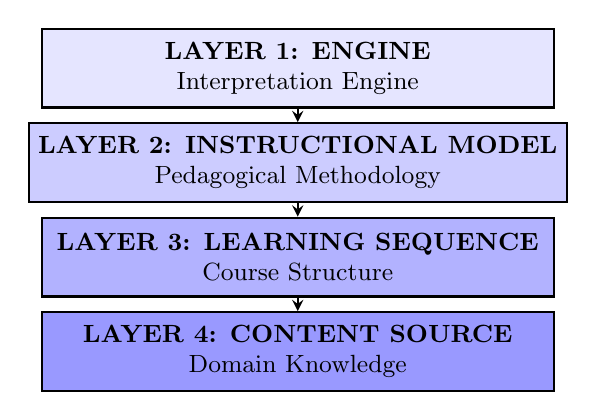
\begin{tikzpicture}[
    layer/.style={
        rectangle,
        draw=black,
        thick,
        minimum width=6.5cm,
        minimum height=1cm,
        align=center,
        font=\small
    }
]

\node[layer, fill=blue!10] (engine) at (0,3.6) {\textbf{LAYER 1: ENGINE}\\Interpretation Engine};

\node[layer, fill=blue!20] (model) at (0,2.4) {\textbf{LAYER 2: INSTRUCTIONAL MODEL}\\Pedagogical Methodology};

\node[layer, fill=blue!30] (sequence) at (0,1.2) {\textbf{LAYER 3: LEARNING SEQUENCE}\\Course Structure};

\node[layer, fill=blue!40] (content) at (0,0) {\textbf{LAYER 4: CONTENT SOURCE}\\Domain Knowledge};

\draw[-stealth, thick] (engine) -- (model);
\draw[-stealth, thick] (model) -- (sequence);
\draw[-stealth, thick] (sequence) -- (content);

\end{tikzpicture}
\caption{TDL four-layer architecture.}
\label{fig:architecture}
\end{figure}

\subsection{Relationship with Classical ITS Architecture}

The TDL architecture can be mapped to the classical ITS architecture, although with important differences:

\begin{table}[h]
\centering
\caption{Correspondence Between ITS and TDL Architecture}
\label{tab:its_tdl_mapping}
\begin{tabular}{@{}ll@{}}
\toprule
\textbf{ITS Component} & \textbf{TDL Layer} \\
\midrule
Domain Model & Content Source (partial) \\
Student Model & \textit{Not implemented} \\
Pedagogical Model & Instructional Model \\
Interface & Engine + LLM platform \\
\bottomrule
\end{tabular}
\end{table}

The absence of a \textit{student model} is a deliberate limitation: TDL does not aim to diagnose the student's cognitive state, but to structure pedagogical interaction coherently. The underlying LLM provides some conversational adaptation, but not the systematic tracking of a traditional ITS.

\subsection{Layer 1: Engine (Interpretation Engine)}

The Engine (current version 1.2) is the most stable component of the architecture. It is implemented as a system prompt loaded into the LLM platform's instruction field. Its function is to teach the model how to interpret and execute TDL files.

The Engine defines four fundamental aspects:

\begin{itemize}
    \item \textbf{Command syntax}: Defines commands such as \texttt{/start} (begin first unit), \texttt{/next} (advance to next unit), and \texttt{/progress} (show current state).

    \item \textbf{State tracking mechanism}: Uses explicit markers with format \texttt{[UNIT:\{id\}|EVENT:\{id\}]} to maintain context between conversation turns.

    \item \textbf{Prompt format}: Specifies how to combine instructional model instructions with learning sequence content.

    \item \textbf{Global behaviors}: Never reveal the system prompt, handle transitions naturally, redirect off-topic conversations back to the study topic.
\end{itemize}

The Engine also establishes the default pedagogical stance: act as a coach rather than a lecturer, verify comprehension before advancing, provide constructive feedback without judgment.

The Engine is modified only when changing the global behavior of all TDL tutors. In practice, it is a component configured once and reused indefinitely.

\subsection{Layer 2: Instructional Model}

The Instructional Model represents teaching methodology as a sequence of instructional events. This concept aligns with Gagn\'{e}'s events of instruction \cite{gagne1985} and represents \textbf{how to teach} in abstract form, independent of specific content.

Each instructional model defines:

\begin{itemize}
    \item \textbf{Name and description}: Identification and explanation of pedagogical philosophy.
    \item \textbf{Event sequence}: Ordered list of steps the tutor must follow.
    \item \textbf{Instructions per event}: What the tutor should do at each event.
    \item \textbf{Transition triggers}: What condition triggers advancement to the next event.
\end{itemize}

An instructional model is completely reusable: the same Bloom 8-Step Interactive model can be applied to a Law course, a Programming course, and a Biology course. Specific content is provided in lower layers.

This concept is functionally analogous to Merrill's \textit{transaction shells} \cite{merrill1991}: reusable pedagogical algorithms for different contents.

\subsection{Layer 3: Learning Sequence}

The Learning Sequence defines the specific structure of a course or lesson. This is where the teacher applies an instructional model to their concrete content.

A learning sequence specifies:

\begin{itemize}
    \item \textbf{Tutor profile}: Knowledge domain, role, style, supported languages.
    \item \textbf{Model inheritance}: Which instructional model to use (via \texttt{extends}).
    \item \textbf{Behaviors}: Initial greeting, help response, off-topic handling, disclaimers.
    \item \textbf{Tools}: Commands available to the student (/start, /progress).
    \item \textbf{Learning units}: Course structure with objectives, event-specific prompts, and navigation between units.
\end{itemize}

The sequence inherits the methodology from the instructional model but provides specific content. This separation is the key to reuse.

\subsection{Layer 4: Content Source}

The Content Source is the subject matter expert's material: notes, texts, references. This layer is optional (sequence prompts can contain content directly), but is especially useful for:

\begin{itemize}
    \item Extensive content that does not fit comfortably in prompts.
    \item Material that is frequently updated (e.g., legal regulations).
    \item Situations where the content expert and instructional designer are different people.
\end{itemize}

TDL supports multiple content source formats: Markdown (recommended), plain text, PDF, Word. The learning sequence references specific content sections via the \texttt{source\_section} field.

\subsection{Data Flow and Interaction}

Fig.~\ref{fig:dataflow} shows how layers interact when a student interacts with a TDL tutor.

\begin{figure}[htbp]
\centering
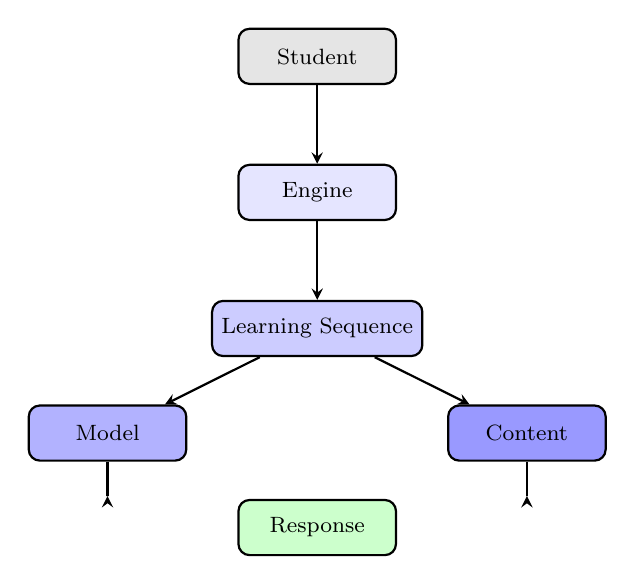
\begin{tikzpicture}[
    node distance=1cm,
    box/.style={
        rectangle,
        draw=black,
        thick,
        rounded corners,
        minimum width=2cm,
        minimum height=0.7cm,
        align=center,
        font=\footnotesize
    }
]

\node[box, fill=gray!20] (user) {Student};
\node[box, fill=blue!10, below=of user] (engine) {Engine};
\node[box, fill=blue!20, below=of engine] (sequence) {Learning Sequence};
\node[box, fill=blue!30, below left=0.6cm and 0.3cm of sequence] (model) {Model};
\node[box, fill=blue!40, below right=0.6cm and 0.3cm of sequence] (content) {Content};
\node[box, fill=green!20, below=1.8cm of sequence] {Response};

\draw[-stealth, thick] (user) -- (engine);
\draw[-stealth, thick] (engine) -- (sequence);
\draw[-stealth, thick] (sequence) -- (model);
\draw[-stealth, thick] (sequence) -- (content);
\draw[-stealth, thick] (model) |- ++(0,-0.8);
\draw[-stealth, thick] (content) |- ++(0,-0.8);

\end{tikzpicture}
\caption{Data flow in TDL.}
\label{fig:dataflow}
\end{figure}

The process follows these steps:

\begin{enumerate}
    \item The student sends a message (e.g., ``Hello'' or \texttt{/start}).
    \item The Engine interprets the message and determines current context (unit, event).
    \item The Engine locates the Learning Sequence in the platform's knowledge base.
    \item The Sequence indicates which Instructional Model to use via \texttt{extends}.
    \item The Engine loads the model's events (E1, E2, ...).
    \item For the current event, the Engine uses model instructions combined with the unit's prompt.
    \item If Content Source is referenced, the Engine incorporates relevant material.
    \item The LLM generates the response following the composed instructions.
    \item The Engine updates state \texttt{[UNIT:id|EVENT:id]} if there is a transition.
\end{enumerate}

\subsection{Separation Principle}

The architecture implements the principle of separation of concerns \cite{merrill1983, merrill1991}:

\begin{itemize}
    \item \textbf{How to execute}: Engine (stable, shared)
    \item \textbf{How to teach}: Instructional Model (reusable across courses)
    \item \textbf{What to teach}: Sequence + Content (course-specific)
\end{itemize}

This separation allows different professionals to contribute to each layer: prompt engineers to the Engine, instructional designers to models, teachers to sequences, and domain experts to content.

% ============================================================================
% V. TDL COMPONENTS AND SPECIFICATION
% ============================================================================
\section{TDL Components and Specification}

This section details the structure and syntax of each TDL component, with illustrative \yamlformat{} code fragments.

\subsection{YAML Specification}

TDL uses \yamlformat{} (YAML Ain't Markup Language) as its serialization format for several reasons:

\begin{itemize}
    \item Human-readable without programming knowledge.
    \item Naturally supports hierarchical structures through indentation.
    \item Allows multiline text for extensive prompts using the \texttt{|} operator.
    \item Widely supported by development tools.
    \item Allows comments for inline documentation.
\end{itemize}

The choice of YAML over XML (used by IMS LD and POML) is based on fewer syntactic characters required: only indentation needs to be understood as a structuring mechanism, without opening/closing tags or escape characters.

\subsection{The Engine: Structure and Functions}

The Engine (current version 1.2) defines command syntax, state tracking mechanism, prompt format, and global behaviors. Its structure includes:

\begin{lstlisting}
engine:
  version: "1.2"
  name: "TDL Engine"
  state_tracking:
    method: "explicit_markers"
    format: "[UNIT:{unit_id}|EVENT:{event_id}]"
  commands:
    start:
      syntax: "/start"
      action: "begin_first_unit"
    next:
      syntax: "/next"
      action: "advance_to_next_unit"
    progress:
      syntax: "/progress"
      action: "show_current_state"
\end{lstlisting}

The Engine also defines security behaviors (never reveal the system prompt), special situation handling (off-topic questions, requests to skip content), and the default pedagogical stance (act as coach, verify comprehension before advancing).

\subsection{Instructional Model: Structure}

An instructional model defines teaching methodology as a sequence of pedagogical events. Each event has an identifier, name, detailed instructions for the LLM, and a trigger that determines when to advance to the next.

\begin{lstlisting}
model:
  id: "bloom-8step-interactive"
  name: "Bloom 8-Step Interactive"
  version: "1.0"
  philosophy: "Never advance without verification"

  events:
    - id: "E1_ACTIVATE"
      name: "Activate Prior Knowledge"
      instructions: |
        Ask what the student knows about
        the topic. Identify correct knowledge,
        misconceptions, and gaps before
        continuing.
      transition_trigger:
        condition: "student_response_received"
        next_event: "E2_OBJECTIVES"

    - id: "E2_OBJECTIVES"
      name: "Present Objectives"
      instructions: |
        Present learning objectives clearly.
        Explain what the student will be
        able to do upon completion.
      transition_trigger:
        condition: "student_response_received"
        next_event: "E3_EXPLAIN"
\end{lstlisting}

\textbf{Transition triggers} define when to advance to the next event, based on:

\begin{itemize}
    \item \texttt{student\_response\_received}: Wait for any student response.
    \item \texttt{comprehension\_verified}: Wait for comprehension verification.
    \item \texttt{explicit\_command}: Wait for explicit command (/next).
    \item \texttt{auto}: Continue automatically without waiting for input.
\end{itemize}

\subsection{Learning Sequence: Structure}

The learning sequence is the file that the teacher creates for their specific course. It inherits from an instructional model via \texttt{extends} and defines tutor profile, behaviors, and learning units.

\begin{lstlisting}
sequence:
  id: "generative-ai-fundamentals"
  name: "Generative AI Fundamentals"
  version: "1.0"
  description: "Tutor for basic concepts
                of Generative AI"
  author: "Pedro Pernias"

  tutor_profile:
    name: "Alex"
    personality: |
      Enthusiastic and patient AI tutor.
      Uses everyday analogies to explain
      technical concepts.
      The Felix example is your favorite
      for explaining attention.
      Never say AI "understands" like humans.

  extends: "instructional_model_bloom.yaml"

  source_content:
    - file: "content_generative_ai.md"
      type: "reference"

  behaviors:
    response_length: "medium"
    language: "en"
\end{lstlisting}

\textbf{Learning units} (\texttt{learning\_units}) structure the course content. Each unit is a discrete topic that passes through all events of the pedagogical model:

\begin{lstlisting}
  learning_units:
    - id: "LU1"
      title: "Foundation Models"
      objectives:
        - level: "understand"
          description: "Explain what a
                        foundation model is"
      prompt: |
        Key points:
        - Large pre-trained models
        - Serve as BASE for many tasks

        Analogy: building foundation.

        Examples: GPT, Claude, LLaMA.
      next: "LU2"

    - id: "LU4"
      title: "Attention Mechanism"
      objectives:
        - level: "understand"
          description: "Explain how attention
                        works"
      prompt: |
        Use the Felix example:
        "Felix saw a black cat and a white
        cat. He gave food to it."

        Problem: What does "it" refer to?
        Solution: Attention allows "looking
        back" to resolve references.
      source_sections:
        - "Section: Transformer Architecture"
      next: "LU5"
\end{lstlisting}

Note that the \texttt{prompt} field is NOT what the tutor says to the student, but an instruction for the tutor about what to teach. It should include: structured key points, concrete examples, suggested analogies, and misconceptions to address.

\subsection{Inheritance Mechanism (extends)}

The \texttt{extends} field allows a learning sequence to inherit methodology from an instructional model. When the Engine processes a sequence with \texttt{extends}:

\begin{enumerate}
    \item Locates the referenced instructional model file.
    \item Loads the model's event sequence (E1, E2, ..., En).
    \item For each learning unit, executes all events in order.
    \item Uses model instructions combined with the unit's prompt.
    \item Manages transitions according to defined triggers.
\end{enumerate}

This mechanism allows the same Bloom 8-Step Interactive model to be applied to completely different courses: the model provides the \textbf{how} (activate prior knowledge, explain, verify, practice) and the sequence provides the \textbf{what} (Foundation Models, Transformers, Attention...).

\subsection{Content Source: Structure}

The content source is a separate file (typically Markdown) containing reference material. It is recommended when:

\begin{itemize}
    \item Content is extensive and does not fit comfortably in prompts.
    \item Material is frequently updated (e.g., legal regulations).
    \item Content expert and instructional designer are different people.
    \item Clear separation of ``what'' from ``how'' is desired.
\end{itemize}

The recommended format uses Markdown with sections delimited by headers:

\begin{lstlisting}
## Section: Foundation Models

Foundation Models are large-scale models
pre-trained with enormous amounts of data.
They serve as a base for multiple
specific tasks...

## Section: Transformer Architecture

The Transformer revolutionized natural
language processing by introducing the
attention mechanism...
\end{lstlisting}

The sequence references specific sections via the \texttt{source\_sections} field:

\begin{lstlisting}
learning_units:
  - id: "LU2"
    title: "Transformer Architecture"
    source_sections:
      - "Section: Transformer Architecture"
    prompt: |
      Explain the Transformer architecture.
      Emphasize that it replaced RNNs.
\end{lstlisting}

The Engine locates the relevant section and incorporates it into context when the prompt requires it. This allows updating content without modifying sequence structure.

\subsection{JSON Schemas for Validation}

To ensure correctness of TDL files, we have developed JSON Schema definitions that specify valid structure for each file type. These schemas enable automatic validation before deployment.

The schema for instructional models verifies:

\begin{itemize}
    \item Presence of required fields (\texttt{model.id}, \texttt{model.events}).
    \item Correct identifier format (lowercase, hyphens).
    \item At least two events in the sequence.
    \item Each event has \texttt{id}, \texttt{instructions}, and \texttt{transition\_trigger}.
\end{itemize}

The schema for learning sequences additionally verifies:

\begin{itemize}
    \item Presence of \texttt{extends} referencing a valid model.
    \item Correct \texttt{tutor\_profile} structure with \texttt{name} and \texttt{personality}.
    \item At least one learning unit defined with \texttt{id}, \texttt{title}, and \texttt{prompt}.
    \item Consistency in \texttt{next} references between units.
\end{itemize}

\subsection{Validation Tool}

We have developed a Python validator that uses JSON Schemas to verify TDL files:

\begin{lstlisting}
pip install tdl-validator
tdl-validate learning_sequence.yaml \
    --model model.yaml
\end{lstlisting}

The validator detects common errors such as missing fields, incorrect types, wrong indentation, or references to non-existent models, providing descriptive messages that facilitate correction.

\subsection{Common Design Patterns}

The TDL manual identifies five common design patterns:

\begin{enumerate}
    \item \textbf{Technical Concepts}: Bloom 8-Step model, frequent verification, everyday analogies, small focused units.

    \item \textbf{Glossary}: Simplified model (Identify, Explain, Connect), no linear sequence, short responses, connections between terms.

    \item \textbf{Practice with Exercises}: Dynamic problem generation, error-type-specific feedback, progressive difficulty.

    \item \textbf{Case Studies}: Contextualized scenarios, guided decision-making, multiple possible paths.

    \item \textbf{Exam Preparation}: Real exam-type questions, detailed answer explanations, weak area identification.
\end{enumerate}

% ============================================================================
% VI. INSTRUCTIONAL MODELS
% ============================================================================
\section{Instructional Models in TDL}

The concept of instructional model is central to TDL. This section elaborates on its theoretical foundation and presents the two reference models included in the specification.

\subsection{The Instructional Event Concept}

Instructional events in TDL are inspired by Robert Gagn\'{e}'s theory \cite{gagne1985}, who identified nine events that optimize learning. TDL adapts this framework to the context of conversational tutoring, where each event represents a phase with a specific pedagogical purpose.

Table~\ref{tab:gagne_mapping} shows the correspondence between Gagn\'{e}'s events and typical TDL events.

\begin{table}[htbp]
\caption{Correspondence Between Gagn\'{e}'s Events and TDL}
\label{tab:gagne_mapping}
\centering
\begin{tabular}{p{3.2cm}p{3.5cm}}
\toprule
\textbf{Gagn\'{e}'s Event} & \textbf{TDL Event} \\
\midrule
Gain attention & Attention / Activate \\
Inform objectives & Objectives \\
Stimulate recall & Recall / Activate \\
Present content & Explain / Present \\
Provide guidance & Guidance / Elaborate \\
Elicit performance & Practice / Elicit \\
Provide feedback & Verify / Feedback \\
Assess performance & Assess \\
Enhance retention & Summary / Transfer \\
\bottomrule
\end{tabular}
\end{table}

This correspondence is not rigid: TDL allows flexibility in how events are organized, as long as they maintain pedagogical coherence.

\subsection{Relationship with Transaction Shells}

TDL's instructional models are functionally analogous to Merrill's \textit{transaction shells} \cite{merrill1991}: reusable pedagogical algorithms for different contents. A transaction shell specifies the sequence of interactions without knowing the specific content; TDL's instructional model does exactly the same.

This analogy reinforces that TDL does not introduce new concepts, but implements established principles in a new technological context (LLMs).

\subsection{Reference Model: Bloom 8-Step Interactive}

The Bloom 8-Step Interactive model implements a Socratic approach where the tutor constantly verifies comprehension before advancing. Its central philosophy is: \textbf{``Never advance without verification.''}

This design aligns with VanLehn's evidence \cite{vanlehn2011}: \textit{step-based} tutors ($d = 0.76$) significantly outperform \textit{answer-based} tutors ($d = 0.31$).

Despite the ``8-Step'' name, the model implements 10 events for greater verification granularity:

\begin{table}[htbp]
\caption{Events of the Bloom 8-Step Interactive Model}
\label{tab:bloom_events}
\centering
\begin{tabular}{clp{2.8cm}}
\toprule
\textbf{ID} & \textbf{Event} & \textbf{Purpose} \\
\midrule
E1 & ACTIVATE & Activate prior knowledge \\
E2 & OBJECTIVES & Present objectives \\
E3 & EXPLAIN & Present content \\
E4 & VERIFY\_EXPLAIN & Verify initial comprehension \\
E5 & ELABORATE & Deepen if correct \\
E6 & VERIFY\_ELABORATE & Verify deepening \\
E7 & PRACTICE & Guided practice \\
E8 & VERIFY\_PRACTICE & Verify practice \\
E9 & SUMMARY & Summary and connections \\
E10 & CLOSE & Closure and transition \\
\bottomrule
\end{tabular}
\end{table}

\subsubsection{Model Characteristics}

\begin{itemize}
    \item \textbf{Continuous verification}: Each explanation (E3, E5) is followed by verification (E4, E6).
    \item \textbf{Immediate feedback}: The tutor evaluates each response before continuing.
    \item \textbf{Cognitive progression}: From recall to comprehension, from comprehension to application, from application to synthesis (aligned with Bloom's taxonomy \cite{anderson2001}).
    \item \textbf{Misconception detection}: E1 identifies incorrect knowledge before teaching.
\end{itemize}

\subsubsection{Ideal Use Cases}

This model is ideal for:

\begin{itemize}
    \item Complex technical concepts where each concept is a prerequisite for the next.
    \item Domains where conceptual errors are costly (medicine, engineering, law).
    \item Students who need active guidance and frequent verification.
    \item Situations where deep understanding is more important than broad coverage.
\end{itemize}

\subsection{Reference Model: Expository}

The Expository model implements a structured lecture approach, based directly on Gagn\'{e}'s nine events. The tutor presents content in an organized manner before requesting active participation.

Its philosophy is: \textbf{``Structured transmission''}---organized presentation with verifications concentrated at the end.

\begin{table}[htbp]
\caption{Events of the Expository Model (based on Gagn\'{e})}
\label{tab:expository_events}
\centering
\begin{tabular}{clp{3cm}}
\toprule
\textbf{ID} & \textbf{Event} & \textbf{Purpose} \\
\midrule
E1 & ATTENTION & Capture initial attention \\
E2 & OBJECTIVES & Inform objectives \\
E3 & RECALL & Stimulate prior recall \\
E4 & PRESENT & Present content \\
E5 & GUIDANCE & Provide guidance \\
E6 & ELICIT & Elicit performance \\
E7 & FEEDBACK & Provide feedback \\
E8 & ASSESS & Assess performance \\
E9 & TRANSFER & Enhance retention \\
\bottomrule
\end{tabular}
\end{table}

\subsubsection{Differences from the Interactive Model}

The key difference is that the tutor can give longer expositions (5--8 paragraphs) before pausing for interaction. The student has a more receptive role initially, with active participation concentrated in E6--E8.

\subsubsection{Ideal Use Cases}

This model is ideal for:

\begin{itemize}
    \item Normative, legal, or regulatory content where precision is critical.
    \item First exposure to a completely new topic.
    \item Rapid coverage of introductory or contextual material.
    \item Students who prefer receiving complete information before interacting.
\end{itemize}

\subsection{Creating Custom Models}

TDL does not limit teachers to reference models. An instructional designer can create custom models following this process:

\begin{enumerate}
    \item Identify the guiding pedagogical philosophy.
    \item Draw the event sequence on paper.
    \item Define what happens in each phase and its purpose.
    \item Define when to advance to the next (triggers).
    \item Write detailed instructions for each event.
\end{enumerate}

For example, the 5E model (Engage, Explore, Explain, Elaborate, Evaluate) for scientific inquiry:

\begin{lstlisting}
model:
  id: "5e-inquiry"
  name: "5E Inquiry Model"
  philosophy: "Discovery through guided
               exploration"

  events:
    - id: "E1_ENGAGE"
      name: "Engage"
      instructions: |
        Capture attention with a provocative
        question or intriguing phenomenon.
        Do NOT reveal the answer yet.
      transition_trigger:
        condition: "student_response_received"
        next_event: "E2_EXPLORE"

    - id: "E2_EXPLORE"
      name: "Explore"
      instructions: |
        Guide the student to discover on
        their own through guiding questions.
        Do NOT give direct answers in
        this phase.
      transition_trigger:
        condition: "exploration_complete"
        next_event: "E3_EXPLAIN"
\end{lstlisting}

Custom model creation opens the possibility of a \textbf{community repository} where instructional designers share validated methodologies that other teachers can apply directly to their courses.

\subsection{Model Limitations}

It is important to recognize the limitations of instructional models in TDL:

\begin{itemize}
    \item \textbf{Predefined sequence}: Models define sequences that repeat for each unit. There is no conditional branching based on student performance.
    \item \textbf{No cognitive diagnosis}: Models do not detect specific misconceptions beyond what the LLM can infer conversationally.
    \item \textbf{LLM dependence}: Execution quality depends on how faithfully the LLM follows instructions. More capable models (GPT-4, Claude 3) produce better results.
\end{itemize}

These limitations are deliberate: they keep TDL simple and portable. More advanced functionalities would require infrastructure that contradicts the goal of deployment on existing commercial platforms.

% ============================================================================
% VII. TECHNICAL SPECIFICATION AND PORTABILITY
% ============================================================================

\section{Technical Specification and Portability}

A key advantage of \tdl{} is its portability: the same files work on multiple LLM platforms without modification. This section describes how this portability is achieved.

\subsection{Cross-Platform Portability}

\tdl{} has been tested on four major platforms. Table~\ref{tab:platforms} shows the configuration for each.

\begin{table}[htbp]
\caption{TDL Configuration by Platform}
\label{tab:platforms}
\centering
\begin{tabular}{lll}
\toprule
\textbf{Platform} & \textbf{Engine} & \textbf{TDL Files} \\
\midrule
ChatGPT GPTs & Instructions & Knowledge \\
Claude Projects & Project Instructions & Project Knowledge \\
Gemini Gems & Instructions & Attached Files \\
OpenWebUI & System Prompt & Knowledge + RAG \\
\bottomrule
\end{tabular}
\end{table}

\subsection{Deployment Process}

The deployment process is consistent across platforms:

\begin{enumerate}
    \item \textbf{Copy the Engine}: The Engine content is copied to the system instructions field (Instructions, System Prompt, or equivalent).

    \item \textbf{Upload TDL files}: The \yamlformat{} files (instructional model and learning sequence) are uploaded to the platform's knowledge area.

    \item \textbf{Upload source content} (optional): If separate source content is used, it is also uploaded to the knowledge area.

    \item \textbf{Configure conversation starters}: Suggested initial messages are configured with ``Hello'' and ``/start''.
\end{enumerate}

\subsection{Platform-Specific Configuration}

\subsubsection{ChatGPT GPTs}

In ChatGPT, custom GPTs have an ``Instructions'' field that accepts up to 8,000 characters. The Engine is copied here. \tdl{} files and source content are uploaded to ``Knowledge,'' where ChatGPT can access them through retrieval.

\begin{lstlisting}
# ChatGPT GPT Configuration
Instructions: [Engine Content]
Knowledge:
  - instructional_model_bloom8.yaml
  - learning_sequence_course.yaml
  - content_course.md
Conversation Starters:
  - "Hello"
  - "/start"
\end{lstlisting}

\subsubsection{Claude Projects}

Claude offers ``Projects'' with project instructions and knowledge files. The Engine is copied to ``Project Instructions.'' \tdl{} files are added as ``Project Knowledge.''

\subsubsection{Gemini Gems}

Google Gemini has ``Gems'' with an instructions field and attached files. The configuration is analogous to the previous platforms.

\subsubsection{OpenWebUI}

OpenWebUI is an open-source interface that can connect to different LLM backends. The Engine is configured as System Prompt, and \tdl{} files are integrated through the platform's RAG (Retrieval Augmented Generation) system.

\subsection{Advantages of Portability}

\tdl{}'s portability offers several advantages:

\begin{itemize}
    \item \textbf{No vendor lock-in}: Institutions can migrate between platforms without rewriting their specifications.

    \item \textbf{Model comparison}: The same tutor can be deployed on GPT-4, Claude, and Gemini to compare performance.

    \item \textbf{Redundancy}: If one platform has availability issues, the tutor can be temporarily deployed on another.

    \item \textbf{Use-case selection}: Different courses can use different platforms according to their needs (cost, specific capabilities, institutional policies).
\end{itemize}

\subsection{Portability Limitations}

Despite general portability, some differences exist between platforms:

\begin{itemize}
    \item \textbf{Instruction-following capability}: More advanced models (GPT-4, Claude 3) follow Engine instructions more faithfully than smaller models.

    \item \textbf{Context limits}: Some platforms have more restrictive limits on system prompt size or knowledge content.

    \item \textbf{Retrieval quality}: The quality of information retrieval from knowledge files varies between platforms.

    \item \textbf{Platform-specific features}: Some platforms offer additional capabilities (code interpreter, browsing) that \tdl{} does not currently leverage.
\end{itemize}

\subsection{Deployment Recommendations}

Based on our experience, we offer the following recommendations:

\begin{enumerate}
    \item \textbf{Test on multiple platforms}: Before production deployment, verify behavior on at least two platforms.

    \item \textbf{Use state-of-the-art models}: For complex tutoring, use GPT-4, Claude 3 Opus/Sonnet, or equivalents.

    \item \textbf{Validate before uploading}: Run the \tdl{} validator on all files before deployment.

    \item \textbf{Document configuration}: Maintain a record of which version of which files are deployed on each platform.
\end{enumerate}

\subsection{Support Tools}

The \tdl{} ecosystem includes support tools:

\begin{itemize}
    \item \textbf{Python validator}: Verifies syntax and structure of \tdl{} files.
    \item \textbf{Reference templates}: Ready-to-adapt instructional models and example sequences.
    \item \textbf{Documentation}: Complete specification guide and best practices.
\end{itemize}

Future work includes development of a \textbf{TDL Maker}: a visual web tool that allows designing learning sequences through drag-and-drop, automatically generating the \yamlformat{}. This tool would further reduce the entry barrier for teachers unfamiliar with structured text formats.

% ============================================================================
% VIII. ALIGNMENT WITH ADL 2.0
% ============================================================================
\section{Alignment with ADL 2.0}

% TODO: This section will be written after completing the other sections
% Content outline:
% - A. How limitations identified in TDL informed ADL 2.0
% - B. Pedagogical decoupling as a test case
% - C. TDL as an ADL 2.0 Profile
% - D. Implications for other domains

\textit{[Section to be completed]}

% ============================================================================
% IX. DISCUSSION
% ============================================================================

\section{Discussion}

\subsection{What Does TDL Contribute?}

\tdl{} does not introduce novel pedagogical concepts. Its contribution is one of \textbf{pragmatic implementation}: it translates established principles of instructional design into a format that works on commercial LLMs without requiring additional infrastructure.

Specifically, \tdl{} offers:

\begin{itemize}
    \item \textbf{Immediate portability}: The same files work on ChatGPT, Claude, Gemini, and OpenWebUI.

    \item \textbf{Accessible format}: YAML is more readable than XML for non-technical users.

    \item \textbf{Demonstrated reusability}: An instructional model can be applied to multiple courses from different disciplines.

    \item \textbf{Formal specification}: JSON Schemas enable automatic validation.

    \item \textbf{Theory alignment}: Instructional events correspond to established frameworks (Gagn\'{e}, Bloom).
\end{itemize}

\subsection{Comparison with Related Work}

Regarding other prompt structuring languages:

\textbf{PDL (IBM)}: Offers sophisticated technical capabilities (type system, function calls) but is oriented toward developers, not educators. It does not incorporate instructional design concepts.

\textbf{POML (Microsoft)}: Its XML syntax provides great expressiveness but introduces unnecessary complexity for the educational use case. The CSS-like style system is powerful but distant from educators' language.

\textbf{IMS Learning Design}: Conceptually complete but failed in adoption due to ecosystem problems, not conceptual complexity. \tdl{} attempts to learn from this failure by prioritizing simplicity and portability.

\tdl{} occupies a specific niche: it combines \yamlformat{}'s readability with concepts specific to instructional design (events, pedagogical models, learning sequences) that neither PDL nor POML contemplate.

\subsection{Implications for Instructional Design Practice}

\tdl{}'s architecture suggests a natural distribution of professional roles:

\begin{itemize}
    \item \textbf{Senior instructional designer}: Creates and validates reusable instructional models. Requires deep knowledge of learning theories.

    \item \textbf{Teacher / Course designer}: Creates learning sequences applying existing models. Requires content knowledge and basic \yamlformat{} familiarity.

    \item \textbf{Content expert}: Creates and updates source content. Only requires subject matter expertise.
\end{itemize}

This separation enables efficient collaboration: an instructional designer can create a ``Problem-Based Learning'' model that teachers in Medicine, Engineering, and Law then use, each with their specific content.

\subsection{Ethical Considerations}

\tdl{} keeps the teacher as author and ultimate responsible party for the educational process. The LLM executes what the teacher has specified, preserving pedagogical authorship. \yamlformat{}'s transparency allows any observer to inspect exactly what methodology the tutor follows.

However, concerns persist:

\begin{itemize}
    \item \textbf{LLM biases}: The underlying model may introduce biases not specified in \tdl{}.

    \item \textbf{Technological dependency}: Students may develop expectations of continuous availability that human tutors cannot satisfy.

    \item \textbf{Privacy}: Conversations with the tutor are processed on third-party servers (OpenAI, Anthropic, Google).
\end{itemize}

\subsection{Limitations}

We acknowledge several limitations of \tdl{} in its current state:

\textbf{Dependence on the underlying LLM}: \tdl{} assumes the LLM will faithfully follow Engine instructions and prompts. In practice, models may occasionally deviate, especially in long conversations.

\textbf{Learning curve for YAML}: Although \yamlformat{} is more readable than other formats, it still requires attention to indentation and syntax. A visual editor that generates \yamlformat{} automatically would facilitate adoption.

\textbf{Improvised pedagogies}: \tdl{} is optimized for structured methodologies with predefined sequences. Highly improvised or emergent approaches may not benefit as much from formalization.

\textbf{Absence of empirical evaluation}: This paper presents \tdl{} as architecture and specification. Empirical validation with real students is planned but not yet executed.

\textbf{Absence of student model}: \tdl{} does not implement a student model. There is no cognitive diagnosis, misconception tracking, or adaptation based on learner history.

\subsection{Risks Inherited from IMS LD}

The history of IMS Learning Design suggests caution. Despite its conceptual soundness, IMS LD did not achieve widespread adoption. \tdl{} mitigates some of the identified risks:

\begin{itemize}
    \item \textbf{Ecosystem}: \tdl{} does not require special tools; any text editor suffices.
    \item \textbf{Portability}: \tdl{} works on multiple platforms without modification.
    \item \textbf{Terminology}: \tdl{} uses familiar terms (events, prompts, units).
\end{itemize}

However, \tdl{} inherits the fundamental risk that the formalization effort may not be perceived as proportional to the benefit obtained. Only empirical validation will determine whether teachers adopt \tdl{} in practice.

\subsection{What TDL Is Not}

It is important to reiterate what \tdl{} does not claim to be:

\begin{itemize}
    \item \tdl{} \textbf{is not a complete ITS}: It lacks the diagnostic and adaptation components that define traditional ITS.

    \item \tdl{} \textbf{does not guarantee effectiveness}: A poorly designed \tdl{} tutor will be as ineffective as any other poorly designed instruction.

    \item \tdl{} \textbf{does not replace the teacher}: The teacher remains the author of pedagogical design; \tdl{} only formalizes and scales their expertise.

    \item \tdl{} \textbf{does not solve LLM limitations}: If the underlying model cannot follow complex instructions, \tdl{} cannot compensate.
\end{itemize}

% ============================================================================
% X. CONCLUSIONS AND FUTURE WORK
% ============================================================================

\section{Conclusions and Future Work}

\subsection{Summary of Contributions}

This paper has presented \tdl{} (Tutor Description Language), an evolution of \adl{} that implements a four-layer architecture for LLM-based tutoring systems. The main contributions are:

\begin{enumerate}
    \item \textbf{Decoupled architecture}: Separation of Engine, Instructional Model, Learning Sequence, and Content Source, enabling independent evolution and reuse.

    \item \textbf{Instructional model as explicit component}: Formalization of ``how to teach'' as a sequence of reusable instructional events, aligned with Gagn\'{e} and Bloom theories.

    \item \textbf{Methodology-content separation}: The same instructional model can be applied to courses from different disciplines; the same content can be taught with different methodologies.

    \item \textbf{Documented evolution from ADL 1.0}: Analysis of ADL~1.0 limitations for tutoring and design principles that guided \tdl{}.

    \item \textbf{Formal specification and tools}: JSON Schema schemas and Python validator to ensure correctness before deployment.

    \item \textbf{Cross-platform portability}: The same \tdl{} files work on ChatGPT, Claude, Gemini, and OpenWebUI without modification.

    \item \textbf{Alignment with ADL~2.0}: Demonstration that \tdl{} can be expressed as an ADL~2.0 profile, validating both the chronological development path and ADL~2.0's extensibility mechanisms.
\end{enumerate}

\tdl{} does not claim to be conceptually novel, but pragmatically useful: an accessible implementation of established principles, adapted to the reality of current LLMs.

\subsection{Research Agenda}

Empirical validation of \tdl{} requires answering specific research questions:

\begin{itemize}
    \item \textbf{RQ1}: Do \tdl{} tutors produce greater learning gains than LLMs without formal pedagogical structure?
    \item \textbf{RQ2}: Does \tdl{} reduce teaching load while maintaining or improving the quality of individualized attention?
    \item \textbf{RQ3}: Can teachers without advanced technical training create functional \tdl{} tutors in reasonable time?
    \item \textbf{RQ4}: Which instructional models are most effective for which types of content and student population?
\end{itemize}

\subsection{Hypotheses}

Based on the reviewed literature, we propose the following hypotheses:

\begin{itemize}
    \item \textbf{H1}: \tdl{} tutors with the Bloom 8-Step model will produce greater learning gains than LLMs with generic prompts, for technical content.

    \item \textbf{H2}: Teachers with deployed \tdl{} tutors will report less time spent on repetitive individualized attention.

    \item \textbf{H3}: Teachers without prior experience will achieve functional \tdl{} tutors in less than 2 hours of work.

    \item \textbf{H4}: Interactive models will be preferred for conceptual content; expository models for normative content.
\end{itemize}

\subsection{Proposed Experimental Design}

We plan a quasi-experimental study during the 2025-2026 academic year with three conditions:

\begin{enumerate}
    \item \textbf{TDL group}: Students with access to a \tdl{} tutor using the Bloom 8-Step model.
    \item \textbf{Generic LLM group}: Students with access to ChatGPT/Claude with a basic prompt.
    \item \textbf{Control group}: Students with traditional materials (notes, videos).
\end{enumerate}

Metrics:

\begin{itemize}
    \item Normalized gain pre-post on knowledge tests.
    \item Self-reported study time.
    \item Engagement (number and depth of interactions with the tutor).
    \item Student satisfaction (Likert scale).
    \item Teaching load (hours dedicated to individualized attention).
\end{itemize}

\subsection{Future Work}

We identify several directions for future work:

\textbf{Visual editor (TDL Maker)}: Development of a web tool that allows designing learning sequences visually, automatically generating the \yamlformat{}. This would eliminate the syntactic barrier for teachers without technical experience.

\textbf{Learning analytics}: Integration of hooks to record which events are executed, student response times, interaction patterns, and dropout points. This data would inform iterative improvement of models and sequences.

\textbf{Community repository}: Creation of an open repository of validated instructional models, where designers can share methodologies and teachers can discover models appropriate for their needs.

\textbf{Assessment extensions}: Adding sections for evaluation rubrics, grading criteria, and automatic generation of student progress reports.

\textbf{Lightweight student model}: Exploring the feasibility of incorporating a simplified student model, leveraging LLMs' conversational memory or external storage, to enable some history-based adaptation.

\textbf{LMS integration}: Developing connectors to integrate \tdl{} tutors with learning management systems (Moodle, Canvas), enabling authentication, progress tracking, and grade synchronization.

\textbf{ADL~2.0 profile formalization}: Completing the formal definition of TDL as an ADL~2.0 profile, including schema definitions and validation rules that ensure compliance with both specifications.

\subsection{Final Conclusion}

The promise of scaling personalized education through AI will not be fulfilled solely with more powerful language models. It requires methods for educators to transfer their pedagogical expertise to these systems. \tdl{} offers a pragmatic path toward this goal: it allows ``how to teach'' to be formalized as reusable knowledge while ``what to teach'' remains under the teacher's control.

By separating responsibilities into well-defined layers and aligning with established instructional design theories, \tdl{} facilitates collaboration among instructional designers, teachers, and content experts. The result is a framework that amplifies educators' impact without compromising their pedagogical authorship.

The alignment with ADL~2.0 validates \tdl{}'s architectural decisions as instances of sound software engineering principles, while simultaneously demonstrating that ADL~2.0's extensibility mechanisms are sufficient for real-world domain specializations. This bidirectional validation strengthens confidence in both specifications.

Empirical validation will determine whether the lessons of the past (particularly from IMS Learning Design) have been learned. \tdl{} is a proposal in that direction, subject to experimental scrutiny and iterative improvement.


% ============================================================================
% ACKNOWLEDGMENTS
% ============================================================================

\section*{Acknowledgments}
This work was partially funded by project AI4ProSa.

% ============================================================================
% BIBLIOGRAPHY
% ============================================================================

% ============================================================================
% BIBLIOGRAFÍA
% ============================================================================

\begin{thebibliography}{00}

\bibitem{bloom1984}
B. S. Bloom, ``The 2 sigma problem: The search for methods of group instruction as effective as one-to-one tutoring,'' \emph{Educational Researcher}, vol. 13, no. 6, pp. 4--16, 1984.

\bibitem{vanlehn2011}
K. VanLehn, ``The relative effectiveness of human tutoring, intelligent tutoring systems, and other tutoring systems,'' \emph{Educational Psychologist}, vol. 46, no. 4, pp. 197--221, 2011.

\bibitem{kulik2016}
J. A. Kulik and J. D. Fletcher, ``Effectiveness of intelligent tutoring systems: A meta-analytic review,'' \emph{Review of Educational Research}, vol. 86, no. 1, pp. 42--78, 2016.

\bibitem{ma2014}
W. Ma, O. O. Adesope, J. C. Nesbit, and Q. Liu, ``Intelligent tutoring systems and learning outcomes: A meta-analysis,'' \emph{Journal of Educational Psychology}, vol. 106, no. 4, pp. 901--918, 2014.

\bibitem{lee2024impact}
D. Lee et al., ``The impact of generative AI on higher education learning and teaching: A study of educators' perspectives,'' \emph{Computers and Education: Artificial Intelligence}, vol. 6, p. 100221, 2024.

\bibitem{kestin2025}
G. Kestin et al., ``AI tutoring outperforms active learning,'' \emph{Nature Human Behaviour}, 2025.

\bibitem{tack2022}
A. Tack and C. Piech, ``The AI teacher test: Measuring the pedagogical ability of blender and GPT-3 in educational dialogues,'' in \emph{Proc. 15th Int. Conf. on Educational Data Mining}, 2022.

\bibitem{macina2023}
J. Macina et al., ``Opportunities and challenges in neural dialog tutoring,'' in \emph{Proc. 16th Int. Conf. on Educational Data Mining}, 2023.

\bibitem{borchers2025}
C. Borchers et al., ``Comparing LLM-based tutors to experienced human tutors,'' in \emph{Proc. Int. Conf. on Artificial Intelligence in Education (AIED)}, 2025.

\bibitem{puech2024}
R. Puech et al., ``Towards pedagogical steering of LLMs for tutoring: A case with productive failure,'' \emph{arXiv preprint arXiv:2410.03781}, 2024.

\bibitem{scarlatos2025}
A. Scarlatos et al., ``Exploring the limitations of LLMs as intelligent tutoring systems,'' \emph{arXiv preprint arXiv:2504.05570}, 2025.

\bibitem{nwana1990}
H. S. Nwana, ``Intelligent tutoring systems: An overview,'' \emph{Artificial Intelligence Review}, vol. 4, no. 4, pp. 251--277, 1990.

\bibitem{woolf2009}
B. P. Woolf, \emph{Building Intelligent Interactive Tutors}. Burlington, MA: Morgan Kaufmann, 2009.

\bibitem{anderson1995}
J. R. Anderson et al., ``Cognitive tutors: Lessons learned,'' \emph{The Journal of the Learning Sciences}, vol. 4, no. 2, pp. 167--207, 1995.

\bibitem{corbett1994}
A. T. Corbett and J. R. Anderson, ``Knowledge tracing,'' \emph{User Modeling and User-Adapted Interaction}, vol. 4, no. 4, pp. 253--278, 1994.

\bibitem{aleven2009}
V. Aleven et al., ``A new paradigm for intelligent tutoring systems: Example-tracing tutors,'' \emph{Int. Journal of Artificial Intelligence in Education}, vol. 19, no. 2, pp. 105--154, 2009.

\bibitem{murray1999}
T. Murray, ``Authoring intelligent tutoring systems: An analysis of the state of the art,'' \emph{Int. Journal of Artificial Intelligence in Education}, vol. 10, pp. 98--129, 1999.

\bibitem{sottilare2012}
R. A. Sottilare et al., ``Design recommendations for intelligent tutoring systems,'' U.S. Army Research Laboratory, 2012.

\bibitem{graesser2004}
A. C. Graesser et al., ``AutoTutor: An intelligent tutoring system with mixed-initiative dialogue,'' \emph{IEEE Transactions on Education}, vol. 48, no. 4, pp. 612--618, 2004.

\bibitem{pardos2024}
Z. A. Pardos and S. Bhandari, ``Learning gain differences between ChatGPT and human tutors-generated hints,'' \emph{PLOS ONE}, vol. 19, no. 3, e0300722, 2024.

\bibitem{merrill1983}
M. D. Merrill, ``Component display theory,'' in \emph{Instructional-Design Theories and Models}, C. M. Reigeluth, Ed. Hillsdale, NJ: Lawrence Erlbaum, 1983, pp. 279--333.

\bibitem{merrill1991}
M. D. Merrill, L. Li, and M. K. Jones, ``Instructional transaction theory: An introduction,'' \emph{Educational Technology}, vol. 31, no. 6, pp. 7--12, 1991.

\bibitem{gagne1985}
R. M. Gagne, \emph{The Conditions of Learning and Theory of Instruction}, 4th ed. New York: Holt, Rinehart and Winston, 1985.

\bibitem{anderson2001}
L. W. Anderson and D. R. Krathwohl (Eds.), \emph{A Taxonomy for Learning, Teaching, and Assessing: A Revision of Bloom's Taxonomy of Educational Objectives}. New York: Longman, 2001.

\bibitem{koper2005}
R. Koper and C. Tattersall (Eds.), \emph{Learning Design: A Handbook on Modelling and Delivering Networked Education and Training}. Berlin: Springer, 2005.

\bibitem{derntl2012}
M. Derntl et al., ``The conceptual structure of IMS Learning Design does not impede its use for authoring,'' \emph{IEEE Transactions on Learning Technologies}, vol. 5, no. 1, pp. 74--86, 2012.

\bibitem{griffiths2005}
D. Griffiths et al., ``Learning design tools,'' in \emph{Learning Design}, R. Koper and C. Tattersall, Eds. Berlin: Springer, 2005, pp. 109--135.

\bibitem{berggren2005}
A. Berggren et al., ``Practical and pedagogical issues for teacher adoption of IMS Learning Design,'' \emph{Journal of Interactive Media in Education}, vol. 2005, no. 1, 2005.

\bibitem{neumann2008}
S. Neumann and R. Oberhuemer, ``User evaluation of a graphical modeling tool for IMS Learning Design,'' in \emph{Proc. 8th Int. Conf. on Advanced Learning Technologies}, IEEE, 2008, pp. 287--291.

\bibitem{ainsworth2002}
S. E. Ainsworth et al., ``Using edit distance algorithms to compare alternative approaches to ITS authoring,'' in \emph{Proc. Int. Conf. on Intelligent Tutoring Systems}, Springer, 2002.

\bibitem{vandeursen2000}
A. van Deursen et al., ``Domain-specific languages: An annotated bibliography,'' \emph{ACM SIGPLAN Notices}, vol. 35, no. 6, pp. 26--36, 2000.

\bibitem{fowler2010}
M. Fowler, \emph{Domain-Specific Languages}. Boston: Addison-Wesley, 2010.

\bibitem{ibm2024pdl}
IBM Research, ``Prompt Declaration Language (PDL),'' 2024. [Online]. Available: https://ibm.github.io/prompt-declaration-language/

\bibitem{zhang2025poml}
Y. Zhang, N. Chen, J. Xu, and Y. Yang, ``Prompt Orchestration Markup Language,'' \emph{arXiv preprint arXiv:2508.13948}, 2025.

\bibitem{pernias2025adl}
P. Pernias et al., ``ADL-based educational assistant architecture: Transforming pedagogical design into automated tutoring systems,'' in \emph{Proc. ICERI 2025}, 2025.

\bibitem{pernias2025adl2}
P. A. Pernías Peco and M. P. Escobar Esteban, ``ADL 2.0: A core specification framework for LLM-based assistants,'' \emph{arXiv preprint}, 2025.

\bibitem{white2023}
J. White et al., ``A prompt pattern catalog to enhance prompt engineering with ChatGPT,'' \emph{arXiv preprint arXiv:2302.11382}, 2023.

\bibitem{reynolds2021}
L. Reynolds and K. McDonell, ``Prompt programming for large language models: Beyond the few-shot paradigm,'' in \emph{CHI 2021 Extended Abstracts}. ACM, 2021, pp. 1--7.

\bibitem{holmes2019}
W. Holmes, M. Bialik, and C. Fadel, \emph{Artificial Intelligence in Education: Promises and Implications for Teaching and Learning}. Boston: Center for Curriculum Redesign, 2019.

\end{thebibliography}


\end{document}
